\section{Partie 2 - Classification}
\subsection{Adapter les données pour la classification}
premièrement nous avons adapter les donnée pour la classification car celles que nous avons collectées étaient faite pour la régression. Par exemple la \textit{feature} \lstinline!delay! a du être modifiée, pour ce faire nous avons créé un script Python. Ce script crée deux fichiers l'un avec les \lstinline!delay! divisé en cinq catégories et le second ou ils sont divisés en seulement trois catégories. Dans le premier cas les catégories sont les suivantes \textit{big late, late, on time, early et big early} et le deuxième cas les trois catégories sont \textit{late, on time et early}. Le script supprime également les valeurs nulles. Pour choisir le meilleurs nombre de classe de \lstinline!delay!, nous avons affiché le nombre d'occurrence de chacune des classes (voir annexe \ref{appendix:3} et annexe \ref{appendix:5} ). On voit qu'il y a moins de \lstinline!delay! dans les classes \textit{big late et big early} et la division des classes est meilleure dans le deuxième cas.

%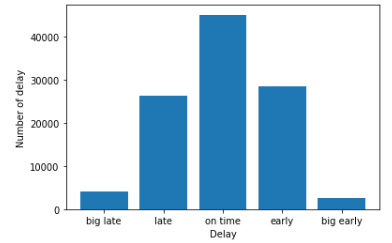
\includegraphics[width=8cm]{images/5.PNG}
%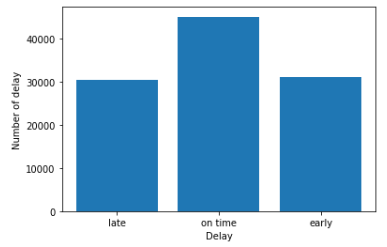
\includegraphics[width=8cm]{images/3.png}

\subsection{Preparation des données pour le machine learning}
Maintenant ce choix fait, nous pouvons aller plus loin, comme l'équipe de régression nous division les données en deux: les assets et les targets. Nous avons ensuite nettoyé les assets pour ne garder que les \textit{features} utile.

\subsubsection{Supprimer les attributes avec toutes les valeurs identiques}

%\includegraphics[width=5cm]{images/all_same.png}

Nous pouvons voir que \lstinline!transport_type, year, month, direction! ont toujours la même valeur pour chaque ligne. Les attributes de type string inutiles ont également été supprimés

%\includegraphics[height=3cm]{images/data_cleaned.PNG}

\subsubsection{Transformation des attributs catégoriels}
Nous transformons les attributes \lstinline!string! utiles en catégorie afin d'aider l'algorithme de machine learning.
%\includegraphics[width=2.5cm]{images/stop_cat.PNG}
%\includegraphics[width=2.5cm]{images/stop_num.PNG}

\subsubsection{Extra feature}
Nous avons également ajouté une colonne supplémentaire qui est la combinaison des colonnes \lstinline!hour! et \lstinline!minute!

%\includegraphics[width=1\textwidth]{images/hour_and_minute.PNG}

\subsection{Selection et entraînement des modèles}
Maintenant que les données sont préparées nous pouvons commencer à choisir et entraîner un modèle. Nous avons pour se faire utilisé différent outils comme la cross-validation ou encore le grid search.

\subsubsection{Decision tree}
Le premier modèle que nous avons testé est l'arbre de décision. Nous avons divisé les données en deux datasets le premier est le test set et le train set. Nous avons choisi le critère d'entropie et le \lstinline!min_sample_leaf = 100! comme hyper paramètres.

Ce qui nous donne un score d'entraînement de 54.4\% et un score de test de 52.2\% avec un 10-folds validation on a une moyenne de 52.4\% and une deviation standard de 0.7\%.

\subsubsection{Random forest}
Nous avons testé 2 random forest:
\begin{itemize}
    \item RandomForestClassifier(n\_estimators=100, criterion="entropy",
    
    bootstrap=True, min\_samples\_leaf=300 class\_weight=class\_weight)
    \item RandomForestClassifier(n\_estimators=100, criterion="entropy",
    
    bootstrap=True, min\_samples\_leaf=100)
\end{itemize}

Le premier nous donne un score d'entraînement de 51.5\% et un score test de 50.6\% nous avons également fait une 10-fold cross validation qui nous donne une moyenne de 50.6\% et une deviation standard de 0.9\%

Le second nous donne un score d'entraînement de 54.0\% et un score test de 52.4\%, le 10-fold cross validation nous donne une moyenne de 52.4\% et une deviation standard de 1.0\%

\subsubsection{KNN}
Nous avons choisi un KNN avec 50 voisins et un \lstinline!leaf_size! de 300. Ce qui nous donne un score d'entraînement de 55.9\% et un score test de 52.6\% avec la 10-fold cross validation on a une moyenne de 53.1\% et une deviation standard de 0.8\%.

\subsubsection{Grid Search pour le random forest}
Nous avons testé une combinaison de 72 hyperparameters \newline
\lstinline!bootstrap= [False,True], n\_estimators = [5,10,100], max\_features = [2, 3, 4,8], min\_samples\_leaf = [100,200,500]! \newline

Le grid search nous indique que la meilleur combinaison est bootstrap = False, max\_features= 8, min\_samples\_leaf =100, n\_estimators =100. \newline
Ce qui nous donne un score d'entraînement de 56.3\% et un score test de 54.1\%.

Si nous regardons de plus près les scores, nous pouvons voir que c'est toujours avec \lstinline!min_sample_leaf = 100! que nous avons les meilleurs résultats donc nous avons testé des valeurs moins grandes.

64 combinaisons d'hyperparameters supplémentaires ont donc été testées.\newline
bootstrap =[False,True], max\_features= [2, 3, 4,8], criterion = ["entropy","gini"], min\_samples\_leaf =  [10,30,50,100] \newline
Selon le grid search les meilleurs paramètres sont: bootstrap = False, criterion = 'entropy', max\_features = 8, min\_samples\_leaf = 10 \newline
Avec un score d'entraînement de 71.5\% et un score test de 58.3\%.

On voit que si on choisit 10 pour \lstinline!min_sample_leaf!, on commence à avoir un petit overfit, selon nous, il faut choisir entre 30 et 50, 30 semblant être le meilleurs. on veut aussi voir que l'indice de gini est le meilleur on peux le supprimer de la grille de recherche.

Nous avons donc décidé de réduire le grid search à 6 combinaison d'hyperparameters.\newline
bootstrap =[False,True], max\_features= [4,8,"auto"]\newline
La meilleur combinaison étant bootstrap = False and max\_features = 8

\subsubsection{Modèle Final}
Notre modèle final est donc un random forest avec comme hyperparameters \lstinline!n_estimator=10, min_sample_leaf=30, bootstrap=False, Max_features=8! Ce qui nous donne un score d'entraînement de 62.3\% et un score test de 56.3\%. \newline
Nous savons que ce n'est pas le meilleur résultat mais ce problème est sûrement lié au manque de données, en ajouter des donnés sur l'état du réseau, les accidents, les travaux, \dots.
